\documentclass[12pt]{extarticle}
\usepackage[utf8]{inputenc}
\usepackage[main=english, spanish]{babel}
\usepackage{csquotes}
\usepackage{graphicx}
\usepackage{fancyhdr}
\usepackage{geometry}
\usepackage{lipsum}
\usepackage{tocloft} 
\usepackage{amsmath}
\numberwithin{equation}{section}
\setlength{\jot}{14pt}
\usepackage{amssymb}
\usepackage{float}
\usepackage{caption}
\usepackage{pifont}
\usepackage[table,xcdraw]{xcolor}
\usepackage{algpseudocode}
\usepackage{algorithm}
\usepackage{booktabs}
\usepackage{multirow}
\usepackage{listings}
\usepackage{subfiles}

\lstset{
  language=Python,
  basicstyle=\ttfamily\scriptsize,
  keywordstyle=\color{blue},
  stringstyle=\color{teal},
  commentstyle=\color{gray}\itshape,
  numbers=left,
  numberstyle=\tiny,
  frame=none,
  captionpos=b,
  breaklines=true,
  showstringspaces=false
}

\definecolor{darkred}{rgb}{0,0,0}
\definecolor{darkgreen}{rgb}{0,0.8,0}
\definecolor{darkblue}{rgb}{0,0,1}

\usepackage[
    backend=biber,
    style=ieee
]{biblatex}

\addbibresource{ref_tfg.bib}
\addbibresource{ref_executive_summary.bib}

\usepackage{hyperref}
\hypersetup{
    colorlinks,
    linkcolor=darkred,
    filecolor=darkblue,
    urlcolor=darkred,
    citecolor=darkgreen
}

% Language-dependent names

\addto\captionsenglish{
    \renewcommand{\contentsname}{Contents}
    \renewcommand{\listfigurename}{List of Figures}
    \renewcommand{\listtablename}{List of Tables}
    \renewcommand{\figurename}{Figure}
    \renewcommand{\tablename}{Table}
    \renewcommand{\lstlistingname}{Algorithm}
    \floatname{algorithm}{Algorithm}
}

% Language-dependent autoref names
\addto\extrasspanish{
    \renewcommand{\tableautorefname}{Tabla}
    \renewcommand{\figureautorefname}{Figura}
    \renewcommand{\equationautorefname}{Ecuación}
    \renewcommand{\sectionautorefname}{Sección}
    \renewcommand{\subsectionautorefname}{Sección}
}

\addto\extrasenglish{
    \renewcommand{\tableautorefname}{Table}
    \renewcommand{\figureautorefname}{Figure}
    \renewcommand{\equationautorefname}{Equation}
    \renewcommand{\sectionautorefname}{Section}
    \renewcommand{\subsectionautorefname}{Section}
}

\newcommand{\blankpage}{
    \clearpage
    \thispagestyle{empty}
    \mbox{}
    \clearpage
}

\usepackage{titlesec}
\usepackage{tocloft}

\titleformat{\section}
  {\normalfont\Large\bfseries}
  {Chapter \thesection}
  {1em}
  {}

\renewcommand{\cftsecpresnum}{Chapter~}
\setlength{\cftsecnumwidth}{6em}

%%%%%%%%%%%%%%%%%%%%%%%%%%%%%%%%%%%%%%%%%%%%%%%%%%%%%%%%%%%%%%%%%%%%%%%%%%%%%%%%%%%%%%%%%%%
%%%%%%%%%%%%%%%%%%%%%%%%%%%%%%%%%%%%%%%%%%%%%%%%%%%%%%%%%%%%%%%%%%%%%%%%%%%%%%%%%%%%%%%%%%%
%% CONFIGURATION
%%%%%%%%%%%%%%%%%%%%%%%%%%%%%%%%%%%%%%%%%%%%%%%%%%%%%%%%%%%%%%%%%%%%%%%%%%%%%%%%%%%%%%%%%%%
%%%%%%%%%%%%%%%%%%%%%%%%%%%%%%%%%%%%%%%%%%%%%%%%%%%%%%%%%%%%%%%%%%%%%%%%%%%%%%%%%%%%%%%%%%%

\newcommand{\projectTitle}{T\'itulo del proyecto}
\newcommand{\projectTitleEnglish}{Title of the project}
\newcommand{\Author}{Student's Name}
\newcommand{\Director}{Supervisor's Name}
\newcommand{\CoDirector}{Deputy Supervisor's Name (if applicable)}
\newcommand{\MonthToSubmit}{May }
\newcommand{\BeginYear}{2025}
\newcommand{\EndYear}{\number\numexpr\BeginYear+1\relax }
%%%%%%%%%%%%%%%%%%%%%%%%%%%%%%%%%%%%%%%%%%%%%%%%%%%%%%%%%%%%%%%%%%%%%%%%%%%%%%%%%%%%%%%%%%%
%%%%%%%%%%%%%%%%%%%%%%%%%%%%%%%%%%%%%%%%%%%%%%%%%%%%%%%%%%%%%%%%%%%%%%%%%%%%%%%%%%%%%%%%%%%

% Title page command
\newcommand{\ComillasTitlePage}{
\begin{titlepage}
    \centering

    
\includegraphics[width=0.35\textwidth]{images/Logo_comillas.png}\\[1cm] 

    {\Huge \textbf{GRADO EN INGENIER\'IA}}\\[0.3cm]
    {\Huge \textbf{MATEM\'ATICA E INTELIGENCIA}}\\[0.5cm]
    {\Huge \textbf{ARTIFICIAL}}\\[1.5cm]

    {\Huge \textbf{TRABAJO FIN DE GRADO}}\\[1.3cm]

    {\huge \projectTitle}\\[0.5cm]

    \vspace{20mm}

    \textbf{Author: \Author}\\[1.0cm]
    \textbf{Director: \Director}\\[0.5cm]
    \textbf{Co-Director: \CoDirector}\\

    \raisebox{-2cm}[0cm][0cm]{\large Madrid, \MonthToSubmit \EndYear}

    \vfill
\end{titlepage}
}

\newcommand{\sectionnotoc}[1]{%
    \refstepcounter{section}%
    \section*{\thesection\quad #1}%
}

\newcommand{\resetcounters}{
    \setcounter{section}{0}
    \setcounter{subsection}{0}
    \setcounter{subsubsection}{0}
    \setcounter{figure}{0}
    \setcounter{table}{0}
    \setcounter{equation}{0}
    \setcounter{footnote}{0}
}

\renewcommand{\sectionmark}[1]{%
    \markright{#1}%
}
%%%%%%%%%%%%%%%%%%%%%%%%%%%%%%%%%%%%%%%%%%%%%%%%%%%%%%%%%%%%%%%%%%%%%%%%%%%%%%%%%%%%%%%%%%%
%%%%%%%%%%%%%%%%%%%%%%%%%%%%%%%%%%%%%%%%%%%%%%%%%%%%%%%%%%%%%%%%%%%%%%%%%%%%%%%%%%%%%%%%%%%

\geometry{top=2.5cm, bottom=4cm, left=2.5cm, right=2.5cm}

\begin{document}

\ComillasTitlePage

\setlength{\headheight}{2cm}

% Configuración del encabezado
\pagestyle{fancy}
\fancyhf{}
\fancyhead[L]{
\includegraphics[width=2cm]{images/Color_logo_comillas.png}} 

\fancyhead[C]{
    \textbf{UNIVERSIDAD PONTIFICIA COMILLAS}\\
    Escuela T\'ecnica Superior de Ingenier\'ia (ICAI)\\
    Grado en Ingenier\'ia Matem\'atica e Inteligencia Artificial
}

\fancyhead[R]{\small\nouppercase{\rightmark}}

\fancyfoot[C]{\thepage}

\newpage

\subfile{Annex_I.tex}

\newpage

{\fontsize{17}{20}
    \begin{center}
        {\large Acknowledgments}
        
    \end{center}
}

\newpage
\captionsetup[figure]{list=false}
\captionsetup[table]{list=false}

\begin{otherlanguage}{spanish}

{\large \MakeUppercase{\projectTitle}}
\vspace{3mm}

\textbf{Autor: \Author}

Director: \Director

Co-Director: \CoDirector

\begin{refsection}[ref_executive_summary.bib]

\section*{Resumen}
\textcolor{red}{Este primer párrafo de resumen deberá tener un máximo de 100 palabras unas 7 líneas.}

\textbf{Palabras clave}: \textcolor{red}{Palabra clave 1}; \textcolor{red}{Palabra clave 2}; .... 

\section*{Resumen ejecutivo}
\textcolor{red}{Este apartado completo debe tener una extensi\'on exacta de 3 p\'aginas y sintetizar el problema abordado, el c\'omo se ha resuelto y los resultados m\'as relevantes obtenidos. Se debe incluir al menos una figura de la arquitectura o diseño de la soluci\'on aportada. Este apartado ser\'a uno de los m\'as importantes, ya que podr\'ia ser la \'unica lectura que una persona que desee conocer por encima el alcance del trabajo realice.}

\sectionnotoc{Introducci\'on}

{\color{red}
\begin{itemize}
    \item \textbf{Contexto:} ¿En qué área se sitúa el trabajo? ¿Qué problema general aborda?
    \item \textbf{Motivación:} ¿por qué es importante resolver este problema?
\end{itemize}
}

\sectionnotoc{Objetivos}

{\color{red}
\begin{itemize}
    \item ¿Qué persigue exactamente tu TFG?
    \item ¿Cuál es la pregunta o hipótesis principal?
\end{itemize}
}

\sectionnotoc{Descripci\'on del modelo/sistema/herramienta}

{\color{red}
\begin{itemize}
    \item ¿Cómo has resuelto el problema?
    \item Herramientas, modelos y técnicas empleadas
\end{itemize}

\begin{figure}[h!]
    \centering
    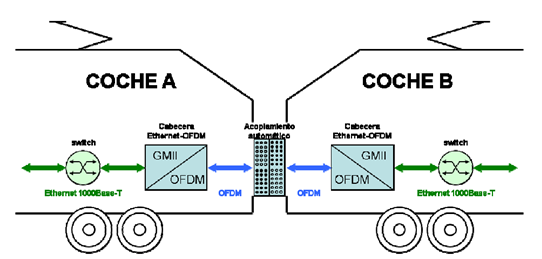
\includegraphics[width=0.5\linewidth]{images/train_schema_example.png}
    \caption{Esquema del sistema conectado de dos vagones contiguos}
    \label{fig:placeholder-es}
\end{figure}

Como se puede ver en la figura \ref{fig:placeholder-es}, ...

}

\sectionnotoc{Resultados}

{\color{red}
\begin{itemize}
    \item ¿C\'omo has validado tu soluci\'on?
    \item ¿Qu\'e resultados has obtenido?
\end{itemize}

\begin{figure}[h!]
    \centering
    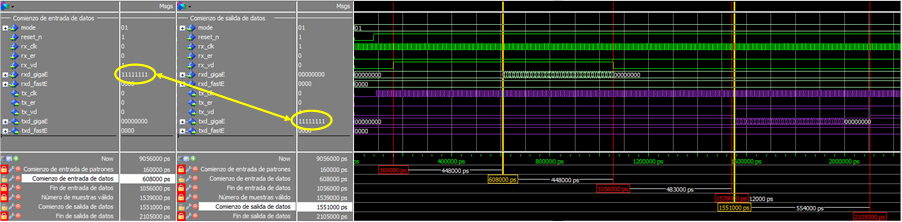
\includegraphics[width=0.5\linewidth]{images/results_example.png}
    \caption{Simulaci\'on del bloque completo de la etapa de frecuencias}
    \label{fig:placeholder2-es}
\end{figure}

Como se puede ver en la figura \ref{fig:placeholder2-es}, ...

}

\sectionnotoc{Conclusiones}

{\color{red}
\begin{itemize}
    \item ¿Qu\'e significan esos resultados?
    \item ¿Cu\'ales son tus principales aportaciones?
\end{itemize}
}

\sectionnotoc{Referencias}

{\color{red}
Incluye las citas necesarias en formato \texttt{bibtex} en el archivo \texttt{ref\_executive\_summary.bib}. Se listar\'an aqu\'i autom\'aticamente seg\'un las utilices usando el comando \texttt{\textbackslash cite} como \cite{einstein1905}.
}

\printbibliography[heading=none]

\end{refsection}

\end{otherlanguage}

\newpage

\resetcounters

%%%%%%%%%%%%%%%%%%%%%%%%%%%%%%%%%%%%%%%%%%%%%%%%%%%%%%%%%%%%%%%%%%%%%%%%%%%%%%%%%%%%%%%%%%%
%% EXECUTIVE SUMMARY IN ENGLISH
%%%%%%%%%%%%%%%%%%%%%%%%%%%%%%%%%%%%%%%%%%%%%%%%%%%%%%%%%%%%%%%%%%%%%%%%%%%%%%%%%%%%%%%%%%%

\begin{otherlanguage}{english}

{\large \MakeUppercase{\projectTitleEnglish}}
\vspace{3mm}

\textbf{Author: \Author}

Director: \Director

Co-Director: \CoDirector

\begin{refsection}[ref_executive_summary.bib]

\section*{Abstract}
\textcolor{red}{This first paragraph of the abstract must have a maximum length of 100 words, approximately 7 lines.}

\textbf{Keywords}: \textcolor{red}{Keyword 1}; \textcolor{red}{Keyword 2}; .... 

\section*{Executive Summary}
\textcolor{red}{This complete section must be exactly 3 pages long and summarize the problem addressed, how it has been solved, and the most relevant results obtained. At least one figure showing the architecture or design of the proposed solution must be included. This section will be one of the most important, since it may be the only section read by someone who wishes to gain a general understanding of the scope of the work.}

\sectionnotoc{Introduction}

{\color{red}
\begin{itemize}
    \item \textbf{Context:} In what area is the work situated? What general problem does it address?
    \item \textbf{Motivation:} Why is it important to solve this problem?
\end{itemize}
}

\sectionnotoc{Objectives}

{\color{red}
\begin{itemize}
    \item What exactly does your Bachelor's Thesis aim to achieve?
    \item What is the main question or hypothesis?
\end{itemize}
}

\sectionnotoc{Description of the Model/System/Tool}

{\color{red}
\begin{itemize}
    \item How have you solved the problem?
    \item Tools, models, and techniques used
\end{itemize}

\begin{figure}[h!]
    \centering
    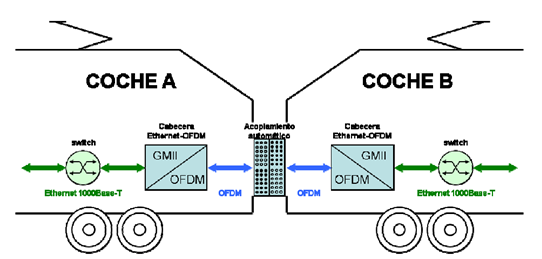
\includegraphics[width=0.5\linewidth]{images/train_schema_example.png}
    \caption{Diagram of the connected system of two adjacent train cars}
    \label{fig:placeholder-en}
\end{figure}

As shown in Figure \ref{fig:placeholder-en}, ...

}

\sectionnotoc{Results}

{\color{red}
\begin{itemize}
    \item How have you validated your solution?
    \item What results have you obtained?
\end{itemize}

\begin{figure}[h!]
    \centering
    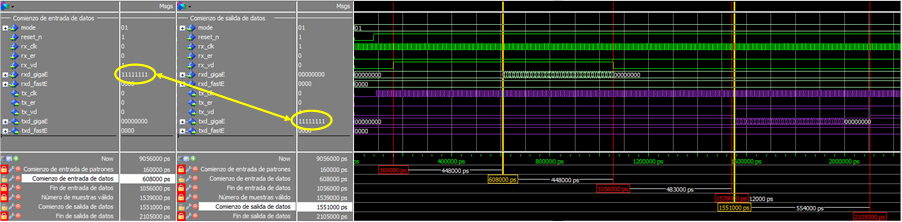
\includegraphics[width=0.5\linewidth]{images/results_example.png}
    \caption{Simulation of the complete block of the frequency stage}
    \label{fig:placeholder2-en}
\end{figure}

As shown in Figure \ref{fig:placeholder2-en}, ...

}

\sectionnotoc{Conclusions}

{\color{red}
\begin{itemize}
    \item What do these results mean?
    \item What are your main contributions?
\end{itemize}
}

\sectionnotoc{References}

{\color{red}
Include the necessary citations in \texttt{bibtex} format in the file \texttt{ref\_executive\_summary.bib}. They will be listed here automatically as you use them with the command \texttt{\textbackslash cite}, as in \cite{einstein1905}.
}

\printbibliography[heading=none]

\end{refsection}

\end{otherlanguage}

\newpage

\captionsetup[figure]{list=true}
\captionsetup[table]{list=true}

\tableofcontents
\thispagestyle{fancy}
\newpage
\setcounter{page}{1}
\fancyfoot[C]{
    \begin{center}
        \thepage
    \end{center}
} 
\renewcommand{\footrulewidth}{0.4pt}
\setlength{\footskip}{0.8cm}

\newpage
\selectlanguage{english}

\phantomsection
\listoffigures

\newpage

\phantomsection
\listoftables

\newpage

%%%%%%%%%%%%%%%%%%%%%%%%%%%%%%%%%%%%%%%%%%%%%%%%%%%%%%%%
%%%% Introduction %%%%%%%%%%%%%%%%%%%%%%%%%%%%%%%%%%%%%%
%%%%%%%%%%%%%%%%%%%%%%%%%%%%%%%%%%%%%%%%%%%%%%%%%%%%%%%%

\resetcounters


\begin{refsection}[ref_tfg.bib]

\section{Introduction}
\textcolor{red}{Introduction goes here}

\textcolor{blue}{Goal of the section: introduce the problem, why this problem should be solved, what improvements carries the solution}

\newpage

%%%%%%%%%%%%%%%%%%%%%%%%%%%%%%%%%%%%%%%%%%%%%%%%%%%%%%%%
%%%% Related works %%%%%%%%%%%%%%%%%%%%%%%%%%%%%%%%%%%%%
%%%%%%%%%%%%%%%%%%%%%%%%%%%%%%%%%%%%%%%%%%%%%%%%%%%%%%%%
\section{State of the Art}\label{sec:related} 
\textcolor{red}{Related work / State of the art goes here}

\textcolor{blue}{Goal of the section: Identify the gap where we are going to develop the solution}

\newpage

%%%%%%%%%%%%%%%%%%%%%%%%%%%%%%%%%%%%%%%%%%%%%%%%%%%%%%%%
%%%%% Objectives %%%%%%%%%%%%%%%%%%%%%%%%%%%%%%%%%%%%%%%
%%%%%%%%%%%%%%%%%%%%%%%%%%%%%%%%%%%%%%%%%%%%%%%%%%%%%%%%
\section{Motivation and Objectives}

\subsection{Motivation}
\textcolor{red}{Why is important to solve/partially solve the gap you have identified}

\textcolor{blue}{Goal of the section: Convince your reader that your project is necessary}

\subsection{Objectives}
\textcolor{red}{List a main objective and at least two secondary objectives}

\textcolor{blue}{Goal of the section: Define what is the exact part of the gap you solve with the project}

\subsection{SDG Alignment}

\textcolor{red}{Of the \href{https://sdgs.un.org/goals}{SDG goals}, list those that your project helps to achieve and justify why.}

\newpage

%%%%%%%%%%%%%%%%%%%%%%%%%%%%%%%%%%%%%%%%%%%%%%%%%%%%%%%%
%%%% Methodology %%%%%%%%%%%%%%%%%%%%%%%%%%%%%%%%%%%%%%%
%%%%%%%%%%%%%%%%%%%%%%%%%%%%%%%%%%%%%%%%%%%%%%%%%%%%%%%%
\section{Methodology}\label{sec:methodology}
\textcolor{red}{Methodology/Developments/Description of the algorithm goes here}

\textcolor{blue}{Goal of the section: Describe in detail the developments done during the projects, including mathematical and programming developments.}

\newpage

%%%%%%%%%%%%%%%%%%%%%%%%%%%%%%%%%%%%%%%%%%%%%%%%%%%%%%%%
%%%% Experiments %%%%%%%%%%%%%%%%%%%%%%%%%%%%%%%%%%%%%%%
%%%%%%%%%%%%%%%%%%%%%%%%%%%%%%%%%%%%%%%%%%%%%%%%%%%%%%%%
\section{Experimental Results}\label{sec:results}

\textcolor{red}{How the algorithm was tested (simulator specification, computing specifications, experiments...), description of evaluation metrics (algorithm accuracy, computing time, ...), use cases, comparison with other methods,...}

\textcolor{blue}{Goal of the section: Proof how well/bad your developments perform with quantitatively and qualitatively}

\newpage

%%%%%%%%%%%%%%%%%%%%%%%%%%%%%%%%%%%%%%%%%%%%%%%%%%%%%%%%
%%%% Conclusions %%%%%%%%%%%%%%%%%%%%%%%%%%%%%%%%%%%%%%%
%%%%%%%%%%%%%%%%%%%%%%%%%%%%%%%%%%%%%%%%%%%%%%%%%%%%%%%%
\section{Conclusions and Future Work}\label{sec:conclusion}
\textcolor{blue}{Goal of the section: Describe how well you have achieved the objectives, in which other fields can your developments be applied, what improvements can be made to the project...}

\newpage

%%%%%%%%%%%%%%%%%%%%%%%%%%%%%%%%%%%%%%%%%%%%%%%%%%%%%%%%
%%%% Referneces  %%%%%%%%%%%%%%%%%%%%%%%%%%%%%%%%%%%%%%%
%%%%%%%%%%%%%%%%%%%%%%%%%%%%%%%%%%%%%%%%%%%%%%%%%%%%%%%%
\section{References} \label{sec:bibliography}
\textcolor{red}{Include the necessary citations in \texttt{bibtex} format in the file \texttt{ref\_tfg.bib}. They will be listed here automatically as you use them with the command \texttt{\textbackslash cite}, as in \cite{einstein1905}.} 

\printbibliography[heading=none]

\end{refsection}
\newpage

%%%%%%%%%%%%%%%%%%%%%%%%%%%%%%%%%%%%%%%%%%%%%%%%%%%%%%%%
%%%% Appendixes %%%%%%%%%%%%%%%%%%%%%%%%%%%%%%%%%%%%%%%%
%%%%%%%%%%%%%%%%%%%%%%%%%%%%%%%%%%%%%%%%%%%%%%%%%%%%%%%%
\appendix

\section{Title of Annex A}
\textcolor{red}{Include as many annexes as necessary. The purpose of the annexes is to include important information that is too extensive to include in the main text of the project (e.g., additional graphs or full tables of experiments/hyperparameters). Ask your supervisor when you are unsure.}



\end{document}




